%%%%%%%%%%%%%%%%%%%%%%%%%%%%%%%%%%%%%%%%%%%%%%%%%%%%%%%%%%%%%%%%%%%%%%%%%%%%%%%%%%%%%%%%%%%%%%%%%%%
\documentclass[11pt]{beamer}
\usetheme[block=fill,progressbar=frametitle]{metropolis}
\usepackage[utf8]{inputenc}
\usepackage[spanish]{babel}
\usepackage{amsmath}
\usepackage{amsfonts}
\usepackage{amssymb}
\usepackage{graphicx}

% numeros con punto decimal, no coma
\decimalpoint

% para la bibliografia
\usepackage[style=verbose,backend=bibtex]{biblatex}
\bibstyle{abbrv}

% codigo de R
\usepackage{listings}
\usepackage{color}

% para las tablitas
\usepackage{booktabs}

% para tablas de colores
\usepackage{xcolor,colortbl}
\usepackage{multirow}

%\usefonttheme[onlymath]{mathserif}
%\usepackage{mathpazo} 
\usepackage{eulervm}                 %
\usepackage[scaled ]{helvet}  

% intento de incluir animaciones
\usepackage{movie15}

%%%%%%%%%%%%%%%%%%%%%%%%%%%%%%%%%%%%%%%%%%%%%%%%%%%%%%%%%%%%%%%%%%%%%%%%%%%%%%%%%%%%%%%%%%%%%%%%%%%

% parametros de sweave
%\SweaveOpts{concordance=TRUE}

%%%%%%%%%%%%%%%%%%%%%%%%%%%%%%%%%%%%%%%%%%%%%%%%%%%%%%%%%%%%%%%%%%%%%%%%%%%%%%%%%%%%%%%%%%%%%%%%%%%

% retoques graficos para el codigo en R
\newsavebox{\caja}

%%%%%%%%%%%%%%%%%%%%%%%%%%%%%%%%%%%%%%%%%%%%%%%%%%%%%%%%%%%%%%%%%%%%%%%%%%%%%%%%%%%%%%%%%%%%%%%%%%%

% comandos para tablas
\newcommand{\bordes}[1]{\renewcommand{\arraystretch}{#1}}
\definecolor{gray}{rgb}{0.5,0.5,0.5}
\definecolor{gris}{gray}{0.925}
\definecolor{gris2}{gray}{0.8}

%%%%%%%%%%%%%%%%%%%%%%%%%%%%%%%%%%%%%%%%%%%%%%%%%%%%%%%%%%%%%%%%%%%%%%%%%%%%%%%%%%%%%%%%%%%%%%%%%%%

% bibliografia
\addbibresource{referencias_estacionariedad.bib}
\addbibresource{referencias_fisiologia.bib}
\addbibresource{referencias_otros.bib}
\addbibresource{referencias_mixto.bib}

\renewcommand{\footnotesize}{\tiny}

%%%%%%%%%%%%%%%%%%%%%%%%%%%%%%%%%%%%%%%%%%%%%%%%%%%%%%%%%%%%%%%%%%%%%%%%%%%%%%%%%%%%%%%%%%%%%%%%%%%

% abreviaciones varias
\newtheorem{defn}{Definición}
\newtheorem{thrm}{Teorema}
\newtheorem{demostracion}{Demostración}
\newtheorem{prop}{Proposición}

\newcommand{\R}{\mathbb{R}}
\newcommand{\intR}{\int_{-\infty}^{\infty}}
\newcommand{\intZ}{\int_{-\infty}^{0}}
\newcommand{\intPI}{\int_{-\pi}^{\pi}}
\newcommand{\simint}[1]{\int_{- #1 }^{ #1 }}
\newcommand{\prima}{^{\prime}}

\newcommand{\ddd}{$\delta$}
\newcommand{\dirac}{$\delta$  de Dirac}

\newcommand{\aste}[1]{\widehat{ #1 }^{\star}}
\newcommand{\est}[1]{\widehat{ #1 }}

\newcommand{\COS}[1]{\mathrm{cos}\left( #1 \right)}
\newcommand{\SEN}[1]{\mathrm{sen}\left( #1 \right)}

\newcommand{\E}[1]{\mathrm{E}\left[ #1 \right]}
\newcommand{\Var}[1]{\mathrm{Var}\left( #1 \right)}
\newcommand{\Cov}[1]{\mathrm{Cov}\left( #1 \right)}
\newcommand{\abso}[1]{\left| #1 \right|}

%%%%%%%%%%%%%%%%%%%%%%%%%%%%%%%%%%%%%%%%%%%%%%%%%%%%%%%%%%%%%%%%%%%%%%%%%%%%%%%%%%%%%%%%%%%%%%%%%%%

% titulo y fecha
\author{Julio Cesar Enciso Alva}
\title{Patrones de homogeneidad espectral en registros polisomnográficos}
\subtitle{Como marcador de posible deterioro cognitivo en adultos mayores}
%\setbeamercovered{transparent} 
\setbeamertemplate{navigation symbols}{} 
%\logo{} 
\institute{Instituto de Ciencias Básicas e Ingeniería\\ 
Universidad Autónoma del Estado de Hidalgo} 
\date{\emph{Neuroscience Short Course}\\
Noviembre de 2017} 
%\subject{} 

%%%%%%%%%%%%%%%%%%%%%%%%%%%%%%%%%%%%%%%%%%%%%%%%%%%%%%%%%%%%%%%%%%%%%%%%%%%%%%%%%%%%%%%%%%%%%%%%%%%

\begin{document}

\begin{frame}
\titlepage
\end{frame}

\begin{frame}
\tableofcontents
\end{frame}

%%%%%%%%%%%%%%%%%%%%%%%%%%%%%%%%%%%%%%%%%%%%%%%%%

%\section{Introducción}

\begin{frame}\frametitle{Motivación}
El estudio y diagnóstico de una gran cantidad de enfermedades depende de nuestra habilidad para
registrar y analizar señales electrofisiológicas. \\

%\vspace{3em}
\vspace{2em}

Se suele asumir que estas señales son complejas: no lineales, \alert{no estacionarias} y sin equilibrio 
por naturaleza. Pero usualmente no se comprueban \textbf{formalmente} estas propiedades.
\end{frame}

%%%%%%%%%%%%%%%%%%%%%%%%%%%%%%%%%%%%%%%%%%%%%%%%%

%\begin{frame}\frametitle{Motivación: formalidad}
%\begin{figure}[h]
%\centering
%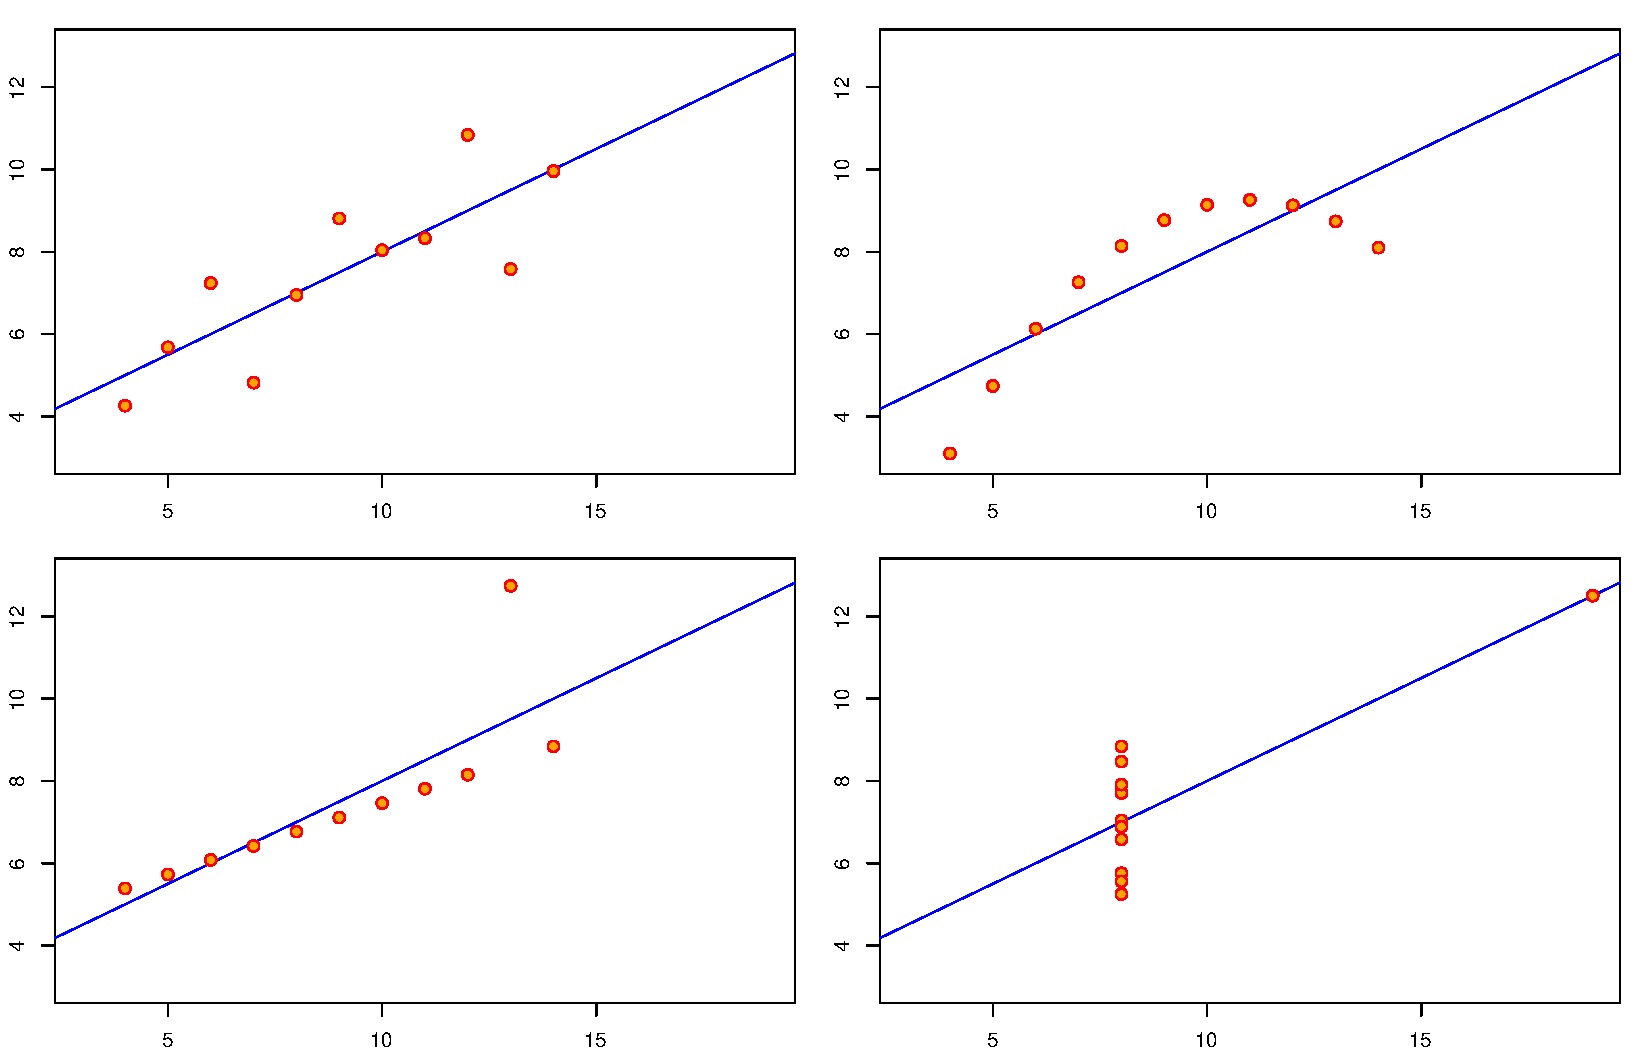
\includegraphics[width=0.9\linewidth]{./img_old/anscombe.pdf} 
%\end{figure}
%\end{frame}

%%%%%%%%%%%%%%%%%%%%%%%%%%%%%%%%%%%%%%%%%%%%%%%%%

\section{Conceptos}

\begin{frame}\frametitle{Conceptos}
\begin{itemize}
\item Promedio $( \mu )$
\item Desviación estándar $( \sigma^{2} )$
\end{itemize}
\begin{figure}
\centering
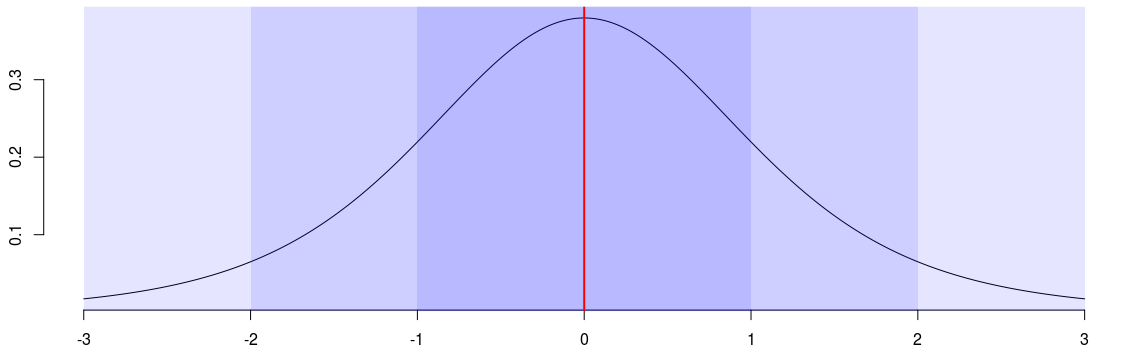
\includegraphics[width=\linewidth]{./curso_scripts/prob.png}
\end{figure}
\end{frame}

%%%%%%%%%%%%%%%%%%%%%%%%%%%%%%%%%%%%%%%%%%%%%%%%%

\begin{frame}\frametitle{Conceptos}
\begin{itemize}
\item Serie de tiempo $\{ X(t) \}$
\end{itemize}
\begin{figure}
\centering
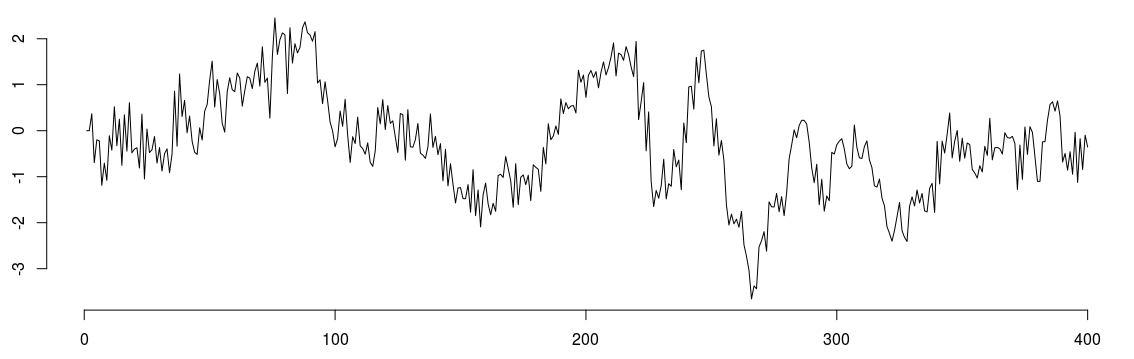
\includegraphics[width=\linewidth]{./curso_scripts/tseries.png}
\end{figure}
\end{frame}

%%%%%%%%%%%%%%%%%%%%%%%%%%%%%%%%%%%%%%%%%%%%%%%%%

\begin{frame}\frametitle{Conceptos}
\begin{itemize}
\item Función de autocorrelación $(\rho)$
\end{itemize}
\begin{figure}
\centering
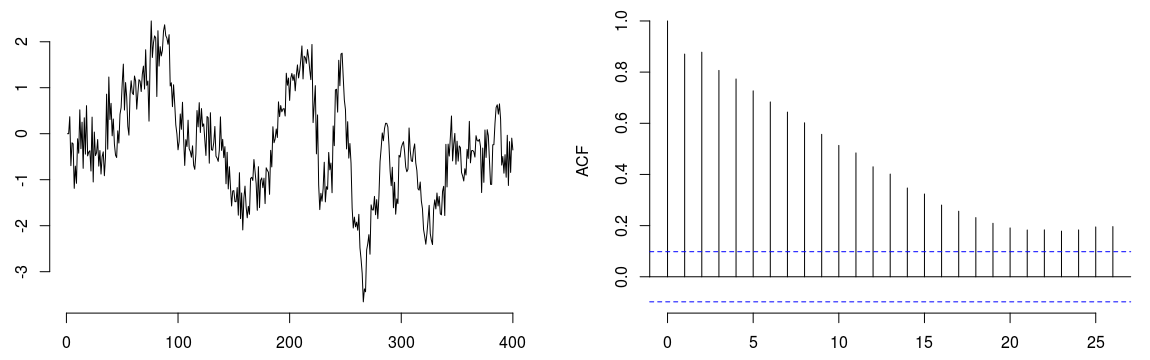
\includegraphics[width=\linewidth]{./curso_scripts/acf.png}
\end{figure}
\end{frame}

%%%%%%%%%%%%%%%%%%%%%%%%%%%%%%%%%%%%%%%%%%%%%%%%%

\begin{frame}\frametitle{Conceptos}
¿ Promedio y desviación estándar de una serie de tiempo ?
\begin{figure}
\centering
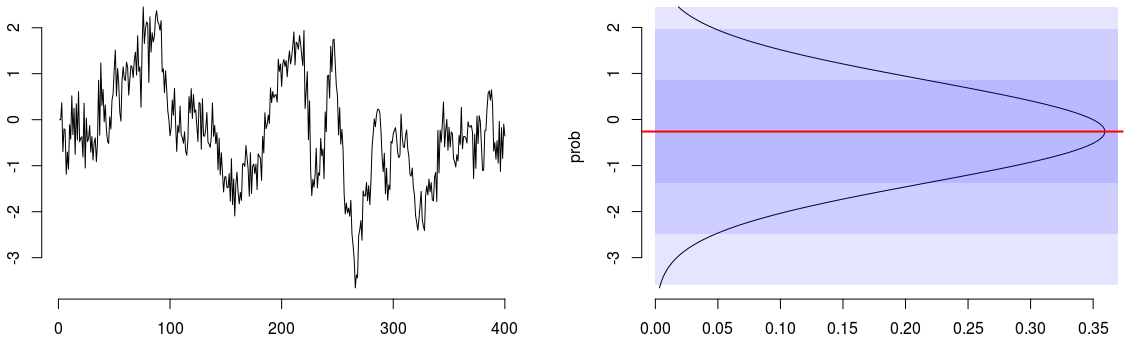
\includegraphics[width=\linewidth]{./curso_scripts/mu_x.png}
\end{figure}
\end{frame}

%%%%%%%%%%%%%%%%%%%%%%%%%%%%%%%%%%%%%%%%%%%%%%%%%

\begin{frame}\frametitle{Conceptos}
¿ Promedio y desviación estándar de una serie de tiempo ?
\begin{figure}
\centering
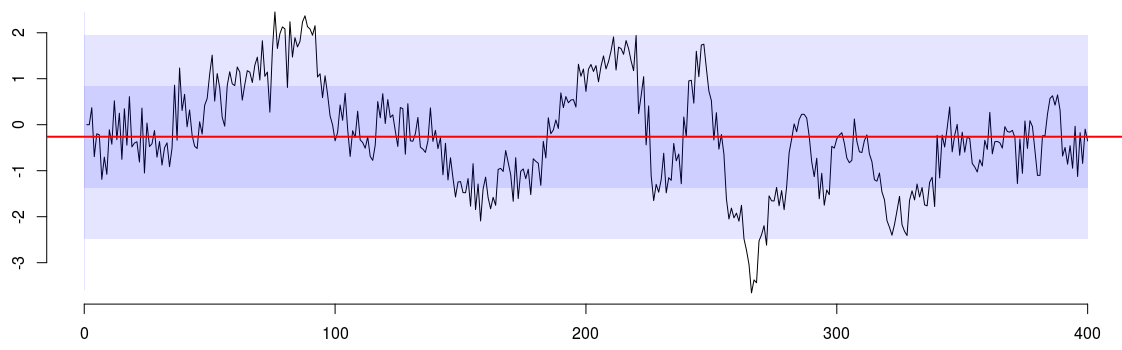
\includegraphics[width=\linewidth]{./curso_scripts/serie_mu.png}
\end{figure}
\end{frame}

%%%%%%%%%%%%%%%%%%%%%%%%%%%%%%%%%%%%%%%%%%%%%%%%%

\begin{frame}\frametitle{Conceptos}
\begin{defn}[Estacionariedad débil]
Un proceso estocástico es débilmente estacionario si y sólo si para cualesquiera tiempos 
admisibles $t$, $s$ se tiene que
\begin{itemize}
\item $\E{X(t)} = \mu_X$
\item $\Var{X(t)} = \sigma^{2}_X$
\item $\Cov{X(t),X(s)} = \rho_X (s-t)$
\end{itemize}
Con $\mu_X$, $\sigma^{2}_X$ constantes, $\rho_X(\tau)$ únicamente depende de $\tau$
\end{defn}
\end{frame}

%%%%%%%%%%%%%%%%%%%%%%%%%%%%%%%%%%%%%%%%%%%%%%%%%

\begin{frame}\frametitle{Un atajo interesante}
Espectro de potencias: 
$f(\omega_j) = \frac{1}{2 T} \simint{T} x(t) e^{-i \omega_j t} dt$
\begin{figure}
\centering
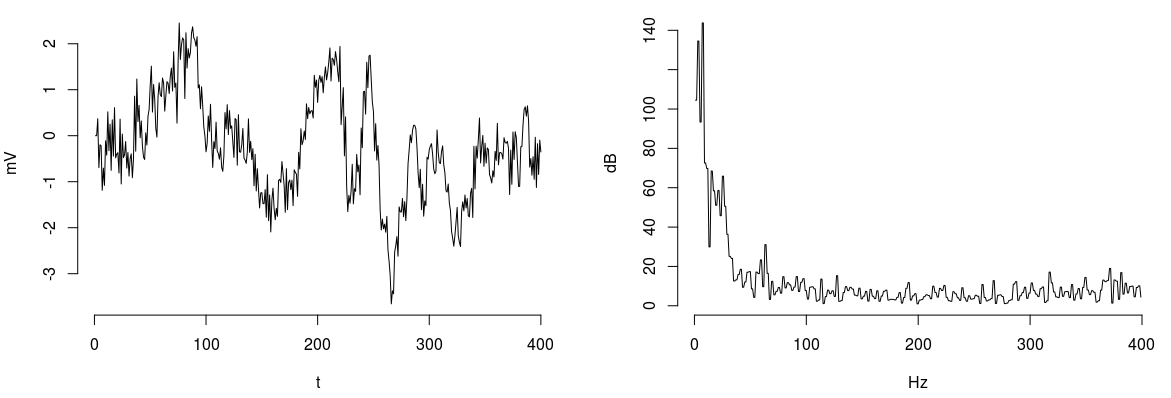
\includegraphics[width=\linewidth]{./curso_scripts/spec.png}
\end{figure}
\end{frame}

%%%%%%%%%%%%%%%%%%%%%%%%%%%%%%%%%%%%%%%%%%%%%%%%%

\begin{frame}\frametitle{Un atajo interesante}
Cantidad de operaciones: $\mathcal{O}(N \log{}N)$ vs $\mathcal{O}(N^{2})$
\begin{figure}
\centering
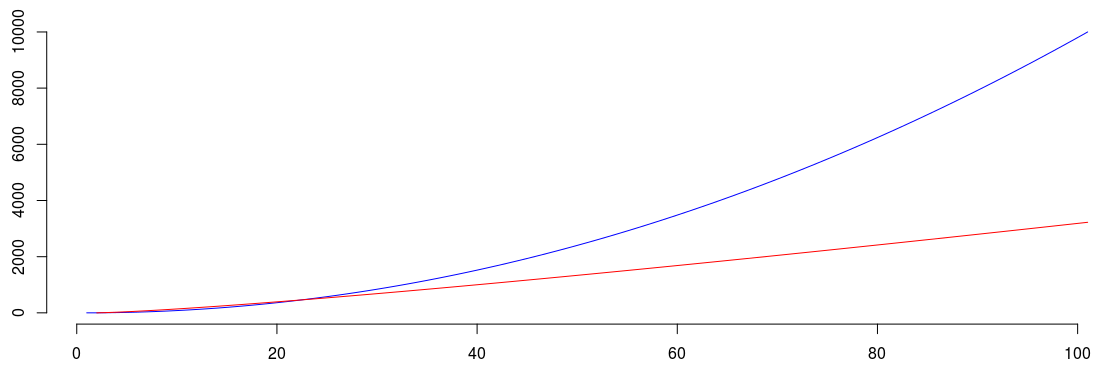
\includegraphics[width=\linewidth]{./curso_scripts/N.png}
\end{figure}
\end{frame}

%%%%%%%%%%%%%%%%%%%%%%%%%%%%%%%%%%%%%%%%%%%%%%%%%

\begin{frame}\frametitle{Espectro de potencias vs Autocorrelación}
\begin{thrm}[Wiener-Khinchin]
Una condición suficiente y necesaria para que $\rho$ sea función de autocorrelación para 
algún proceso a tiempo continuo débilmente estacionario y estocásticamente continuo, 
$\{X(t)\}$,  es que exista una función $F$ tal que
%\begin{itemize}
%\item Es monótonamente creciente
%\item $F(-\infty) = 0$
%\item $F(+\infty) = 1$
%\item Para todo $\tau \in \R$ se cumple que
\begin{equation*}
\rho(\tau) = \intR e^{i \omega \tau} dF(\omega)
\end{equation*}
%\end{itemize}
\end{thrm}
\end{frame}

%%%%%%%%%%%%%%%%%%%%%%%%%%%%%%%%%%%%%%%%%%%%%%%%%

\begin{frame}\frametitle{Espectro de potencias para series no-estacionarias}
Se considerarán procesos no-estacionarios \alert{de media cero y varianza finita} que admitan una 
representación de la forma
\begin{equation*}
X(t) = \intPI A(t,\omega) e^{i t \omega} dZ(\omega)
\end{equation*}
tal que 
\begin{itemize}
\item $\Cov{dZ(\omega),dZ(\lambda)} = 0 \Leftrightarrow \omega \neq \lambda$
\item $\E{\abso{dZ(\omega)}^{2}} = \mu(\omega)$
\end{itemize}

El \textbf{espectro evolutivo} fue definido por Priestley \footcite{Priestley65} como
\begin{equation*}
f(t,\omega) = \abso{A(t,\omega)}^{2}
\end{equation*}
\end{frame}

%%%%%%%%%%%%%%%%%%%%%%%%%%%%%%%%%%%%%%%%%%%%%%%%%

\begin{frame}\frametitle{Base de la prueba de Priestley-Subba Rao}
Supóngase que puede expresarse a $\{X(t)\}$ como
\begin{equation*}
X(t) = \int_{-\pi}^{\pi} A(t,\omega) e^{i\omega t} \, d\xi(\omega)
\end{equation*}

\begin{center}
$\{ X(t) \}$ estacionario $\Rightarrow A(t,\omega)$ constante $\Rightarrow f(t,\omega)$ constante
\end{center}

\pause
%\begin{center}
%$f(t,\omega)$ no-constante $\Rightarrow \{X(t)\}$ \textbf{no} estacionaria
%\end{center}

Prueba de hipótesis para

\begin{center}
$H_0 : f(t,\bullet)$ no depende de $t$
\end{center}
\end{frame}

%%%%%%%%%%%%%%%%%%%%%%%%%%%%%%%%%%%%%%%%%%%%%%%%%

\begin{frame}\frametitle{El estimador de doble ventana}
\begin{defn}[Estimador de doble ventana]
%Se define a $\est{f}$, estimador para la $f$, como
\begin{equation*}
\widehat{f}(t,\omega) = \int_{t-T}^{t} w_{T'}(u) \lvert U(t-u,\omega) \lvert^{2} du
\end{equation*}

Donde $w_{T'}$, $U$, $g$, $\Gamma$ son tales que
\begin{small}
\begin{itemize}
\item $U(t,\omega) = \int_{t-T}^{t} g(u) X({t-u}) e^{i \omega (t-u)} du$
\item $2\pi \int_{-\infty}^{\infty} \lvert g(u) \lvert^{2} du = 
\int_{-\infty}^{\infty} \lvert \Gamma(\omega) \lvert^{2} d\omega = 1$
\item $w_{\tau}(t) \geq 0$ para cualesquiera $t$, $\tau$
\item $w_{\tau}(t) \rightarrow 0$ cuando $\lvert t \lvert \rightarrow \infty$, para todo $\tau$
\item $\int_{-\infty}^{\infty} w_{\tau}(t) dt = 1$ para todo $\tau$
\item $ \int_{-\infty}^{\infty} \left( w_{\tau}(t) \right)^{2} dt < \infty$ para todo $\tau$
%\item Existe un $C$ tal que  
%$\lim_{\tau \rightarrow \infty} \tau \int_{-\infty}^{t} \abso{ W_{\tau}(\lambda) }^{2} d\lambda = C$
\end{itemize}
\end{small}
\end{defn}
\end{frame}

%%%%%%%%%%%%%%%%%%%%%%%%%%%%%%%%%%%%%%%%%%%%%%%%%

\begin{frame}\frametitle{Estimador de doble ventana}
\begin{prop}
El estimador $\widehat{f}$ tiene las siguientes propiedades
\begin{itemize}
\item $\displaystyle \E{\est{f}(t,\omega)} \approx f(t,\omega)$
\item $\displaystyle \Var{\est{f}(t,\omega)} \approx 
\frac{C}{\tau} f^{2}(t,\omega) \intR \abso{\Gamma (\theta)}^{4} d\theta$
\item $\displaystyle \Cov{\est{f}(t_1,\omega_1) , \est{f}(t_2,\omega_2)} \approx $
{\small $\intR \intR
w_\tau (u) w_\tau(v) \Cov{ \abso{U(t_1-u,\omega_1)}^{2} , \abso{U(t_2-u,\omega_2)}^{2} } du dv$
}
\end{itemize}
\end{prop}
\end{frame}

%%%%%%%%%%%%%%%%%%%%%%%%%%%%%%%%%%%%%%%%%%%%%%%%%

\begin{frame}\frametitle{Estimador de doble ventana}
Puede escribirse
$Y(t,\omega) = \log \left( f(t,\omega) \right) + \varepsilon(t,\omega)$, 
donde 
%las variables $\varepsilon(t,\omega)$ satisfacen que
\begin{itemize}
\item $\displaystyle \E{\varepsilon(t,\omega)} = 0$
\item $\displaystyle \Var{\varepsilon(t,\omega)}
\approx \frac{C}{\tau} \intR \abso{\Gamma (\theta)}^{4} d\theta =: \sigma^{2}$
\end{itemize}

Como $f$ y $Y$  dependen (o no) simultáneamente de $t$, se puede usar 
la siguiente prueba de hipótesis
%\begin{equation*}
%\sum_{i = 1 }^{N} \left( Y(t,\omega_i) - \overline{Y}(\bullet,\omega_i) \right)^{2} 
%\sim \sigma^{2} \chi^{2}(N)
%\end{equation*}
\begin{equation*}
H_0 : \sum_{i = 1 }^{N} \left( Y(t,\omega_i) - \overline{Y}(\bullet,\omega_i) \right)^{2} 
= 0
\end{equation*}
con $\overline{Y}(\bullet,\omega) = \frac{1}{M} \sum_{j=1}^{M} Y(t_j,\omega)$
%; el estadístico tiene distribución $\chi^{2}$
\end{frame}

%%%%%%%%%%%%%%%%%%%%%%%%%%%%%%%%%%%%%%%%%%%%%%%%%

\begin{lrbox}{\caja}%
\begin{lstlisting}[caption={}]
Priestley-Subba Rao stationarity Test for datos
-----------------------------------------------
Samples used              : 3072 
Samples available         : 3069 
Sampling interval         : 1 
SDF estimator             : Multitaper 
  Number of (sine) tapers : 5 
  Centered                : TRUE 
  Recentered              : FALSE 
Number of blocks          : 11 
Block size                : 279 
Number of blocks          : 11 
p-value for T             : 0.4130131 
p-value for I+R           : 0.1787949 
p-value for T+I+R         : 0.1801353 
\end{lstlisting}
\end{lrbox}%

%%%%%%%%%%%%%%%%%%%%%%%%%%%%%%%%%%%%%%%%%%%%%%%%%

\begin{frame}[fragile]\frametitle{Resultados de la prueba PSR}
\begin{figure}
\scalebox{0.7}{\usebox{\caja}}
%\caption{La prueba de Priestley-Subba Rao se encuentra implementada en R como la función 
%\texttt{stationarity()}, del paquete \texttt{fractal}}
\end{figure}
\end{frame}

%\begin{frame}[fragile]\frametitle{Espectro estimado}
%
%\begin{center}
%\begin{tabular}{cc}
%%\includemovie{5em}{5em}{./img_old/priestley_spectra_full.gif}
%%\includemovie{5em}{5em}{./img_old/priestley_spectra_small.gif}
%pelis
%\end{tabular} 
%\end{center}
%
%%Por hacer: reescribir las ecuaciones del paper priestley68
%\end{frame}

%%%%%%%%%%%%%%%%%%%%%%%%%%%%%%%%%%%%%%%%%%%%%%%%%

%\begin{frame}[fragile]\frametitle{Espectro estimado}
%\begin{figure}
%\centering
%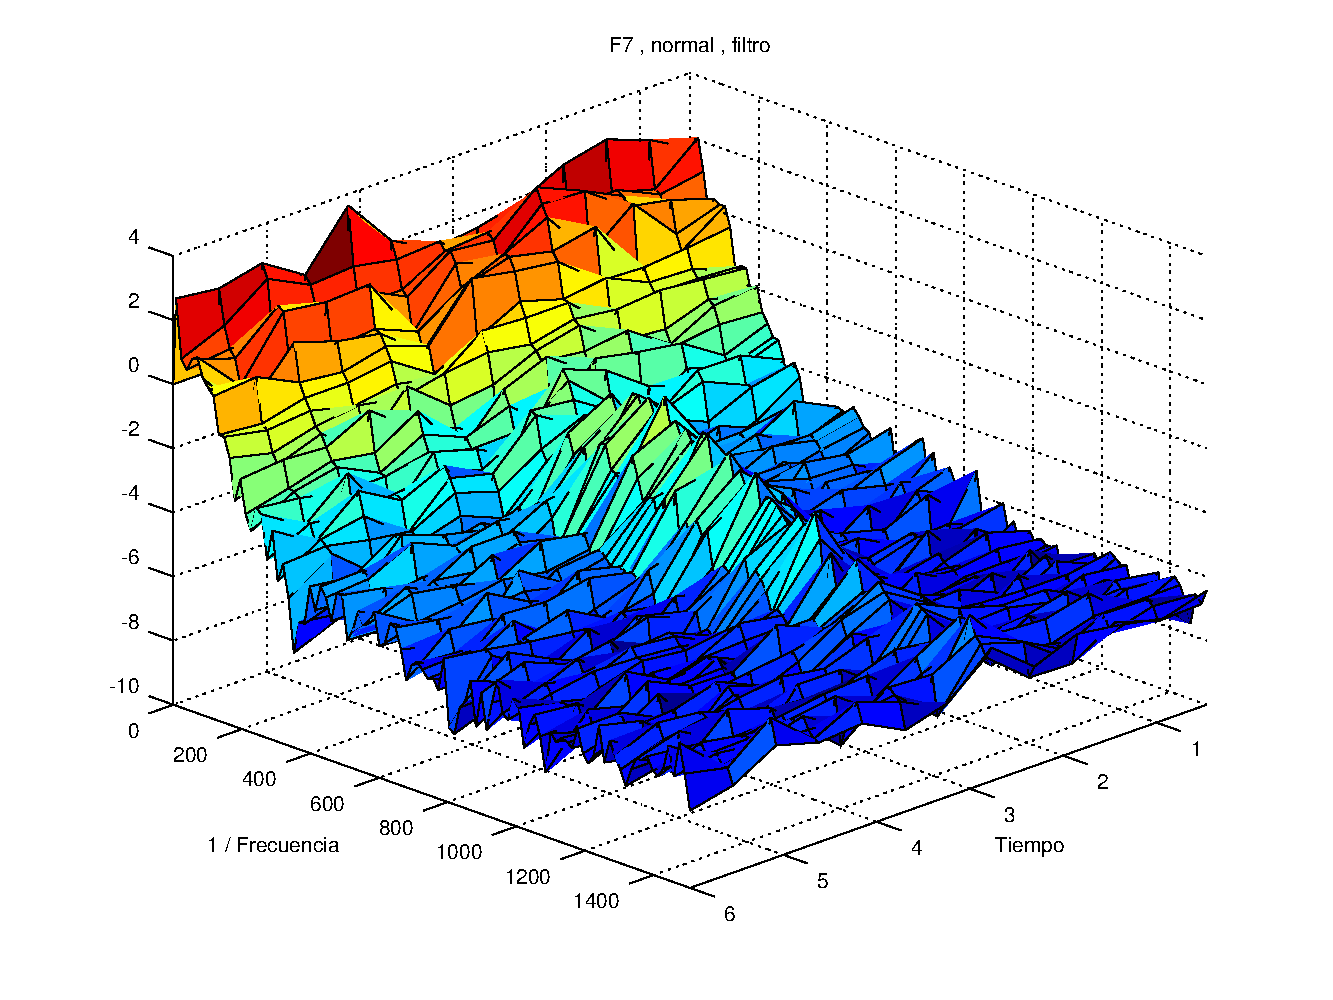
\includegraphics[width=\linewidth]{./img_old/n7f.pdf} 
%\end{figure}
%\end{frame}

%%%%%%%%%%%%%%%%%%%%%%%%%%%%%%%%%%%%%%%%%%%%%%%%%

\begin{frame}\frametitle{Descomposición clásica usando loess}

Filtro no-paramétrico para generar las series de tiempo
\begin{equation*}
X(t) = T(t) + S(t) + R(t)
\end{equation*}\\

Tales que:\\
\begin{description}
\item[$S$] Función periódica suave, comp. estacional
\item[$T$] Función suave, tendencia
\item[$R$] Residuo
\end{description}

%Comando en R: \textcolor{red}{\texttt{stl()}}
\end{frame}

%%%%%%%%%%%%%%%%%%%%%%%%%%%%%%%%%%%%%%%%%%%%%%%%%

%\begin{frame}[fragile]
%\begin{figure}[h]
%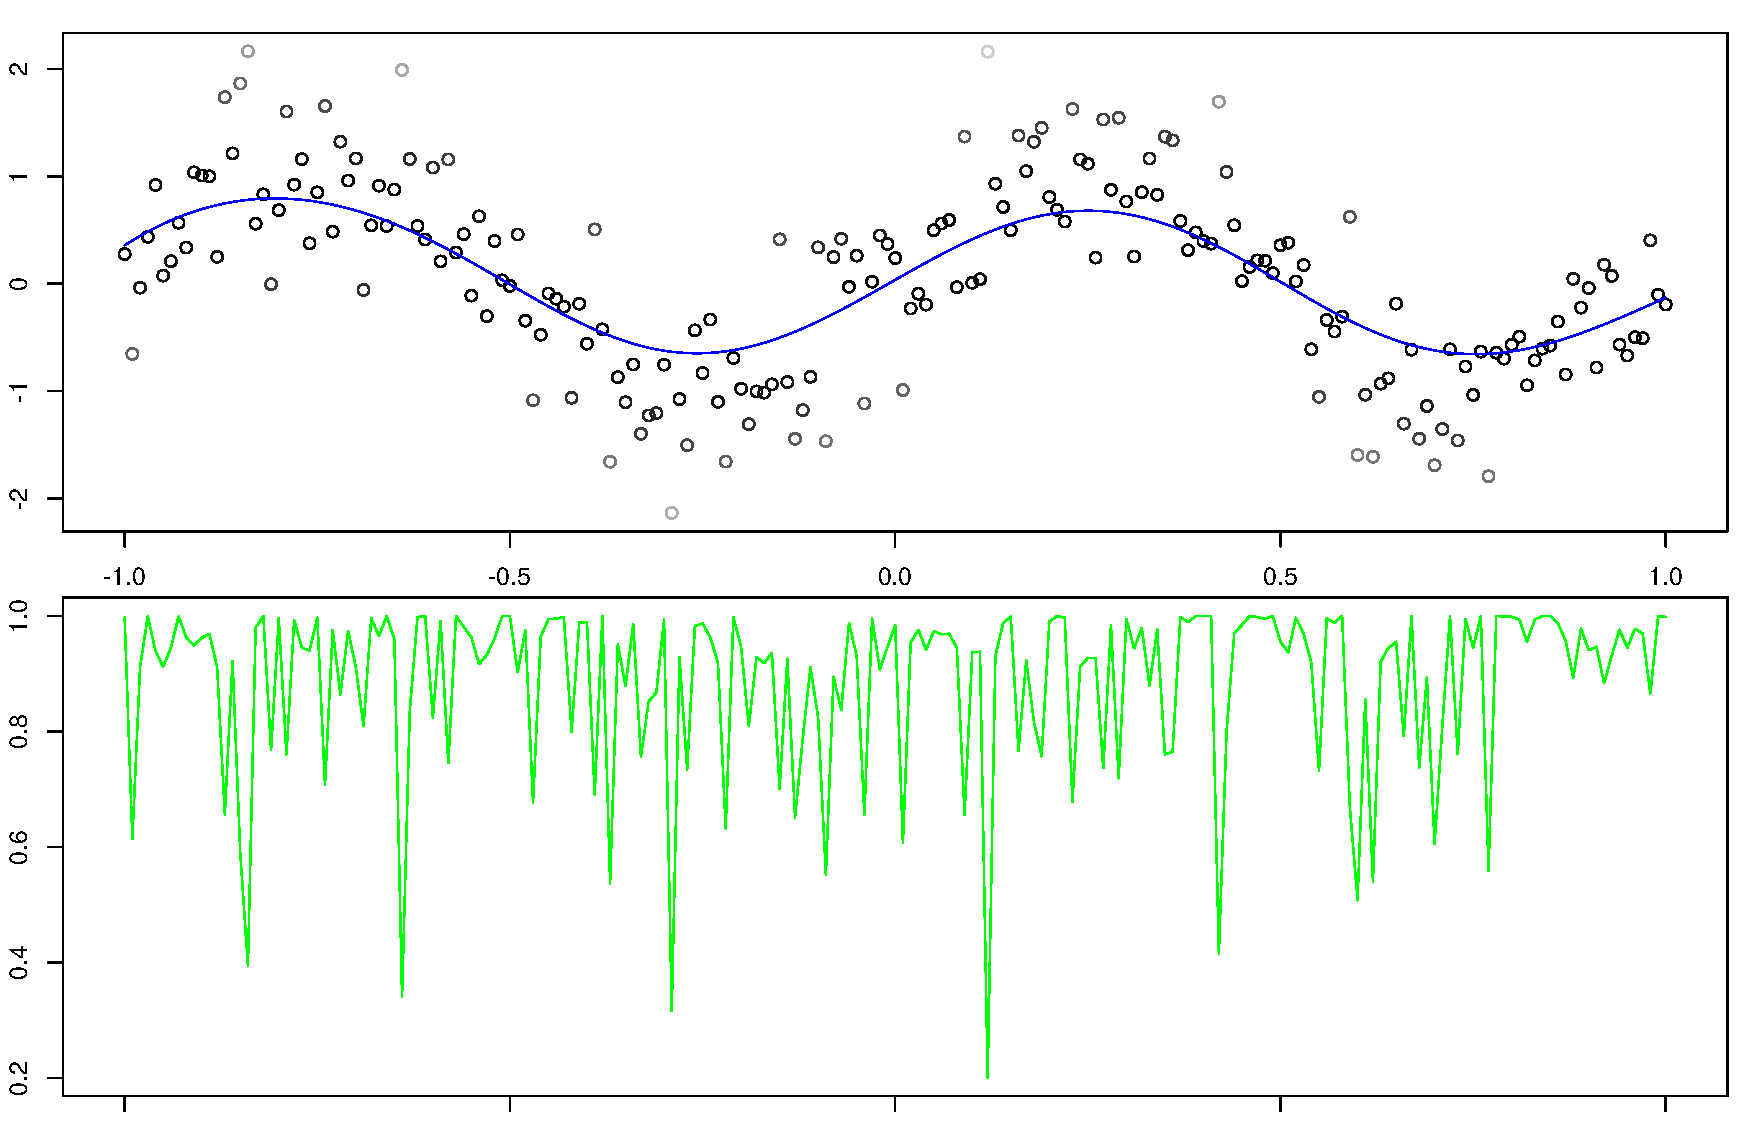
\includegraphics[width=\linewidth]{./img_old/stl_demo2_1.pdf} 
%\end{figure}
%%\begin{center}
%%\includemovie{3em}{3em}{./img_old/stl_demo2_gif.gif}
%%\end{center}
%\end{frame}

%%%%%%%%%%%%%%%%%%%%%%%%%%%%%%%%%%%%%%%%%%%%%%%%%

\section{Ejemplo práctico}

\begin{frame}\frametitle{Software estadístico R}

Lenguaje para cómputo estadístico y graficación; multi- plataforma (Linux, Windows, MacOS), 
de código abierto y acceso gratuito a través de su página
\href{https://www.r-project.org/}{\beamergotobutton{Link}}

\begin{figure}
\centering

\includegraphics[width=0.4\linewidth]{./curso_scripts/r_logo.pdf}
\end{figure}

Por simplicidad, se usará la interfaz gráfica de RStudio
\href{https://www.rstudio.com/}{\beamergotobutton{Link}}
\end{frame}

%%%%%%%%%%%%%%%%%%%%%%%%%%%%%%%%%%%%%%%%%%%%%%%%%

\begin{frame}\frametitle{Datos: registros}
\begin{figure}
\centering
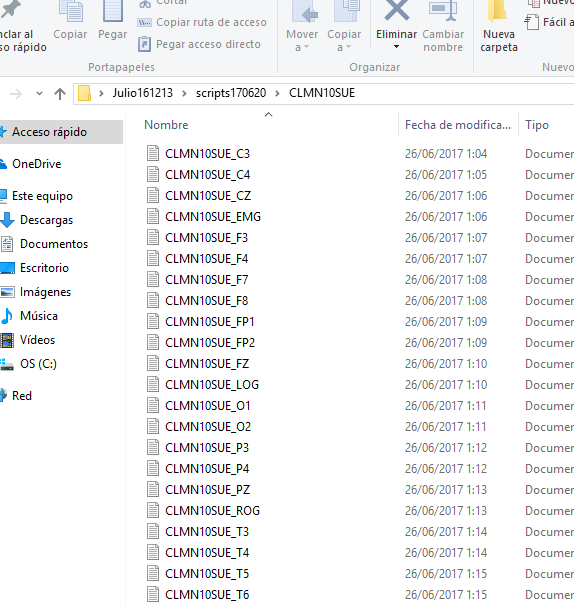
\includegraphics[width=0.7\linewidth]{./curso_scripts/archivos.png}
\end{figure}
\end{frame}

%%%%%%%%%%%%%%%%%%%%%%%%%%%%%%%%%%%%%%%%%%%%%%%%%

\begin{frame}\frametitle{Graficación de los datos}
\begin{figure}
\centering
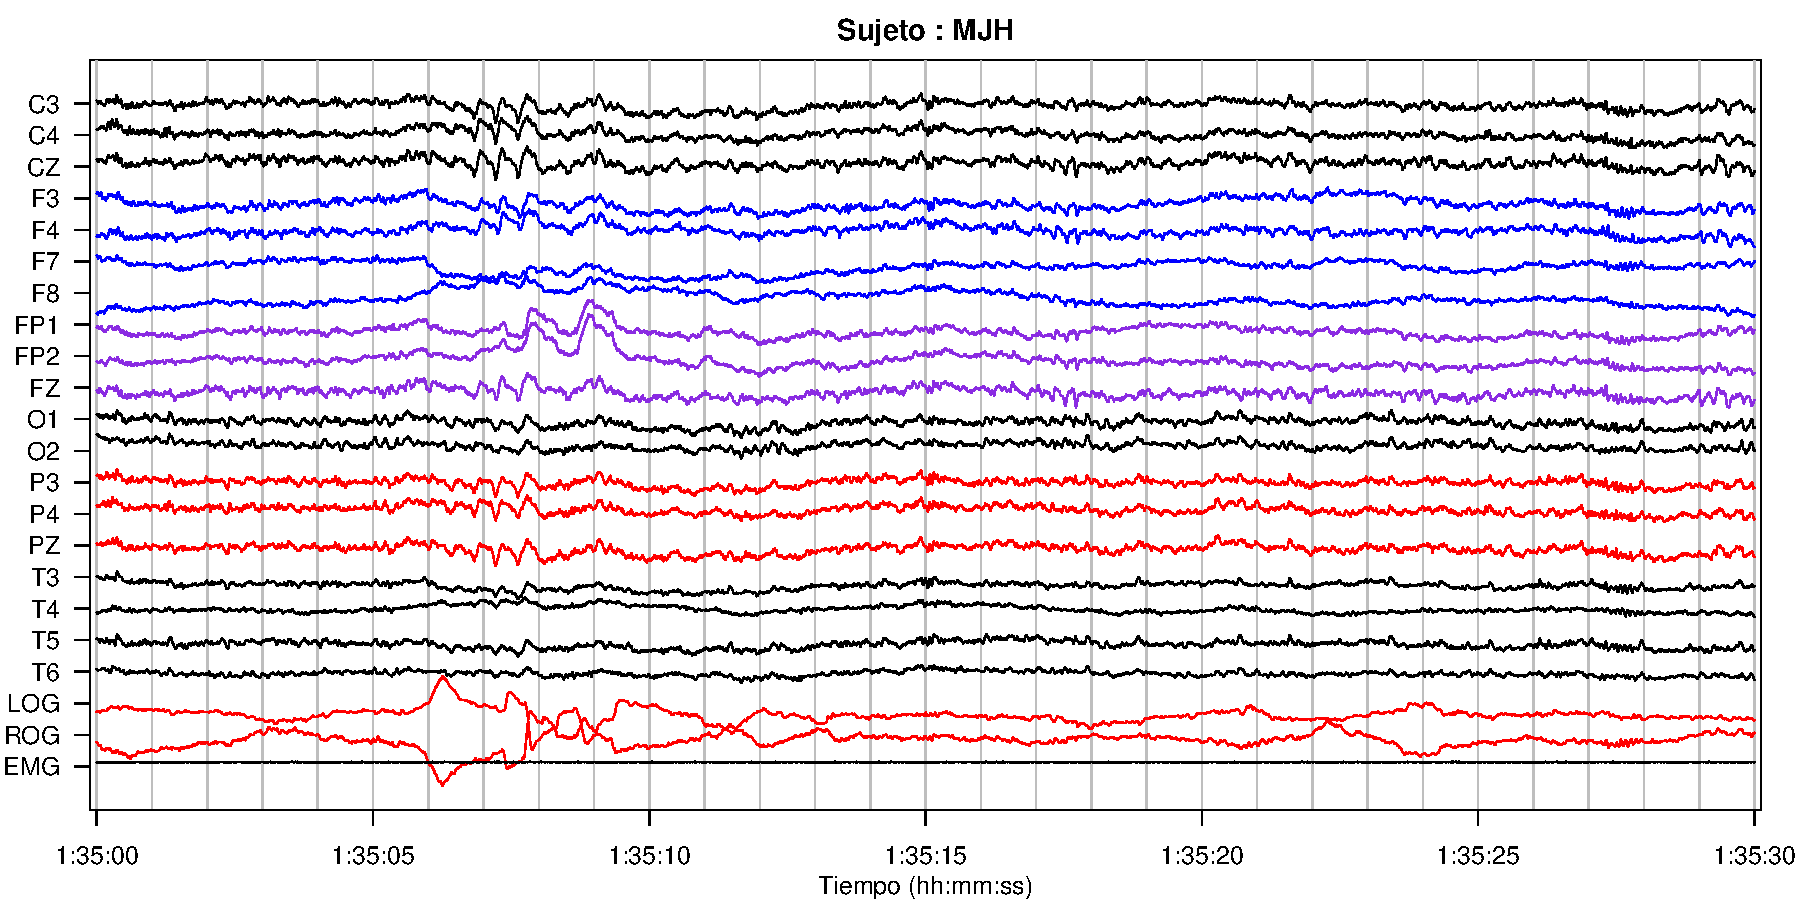
\includegraphics[width=\linewidth]{./img_ejemplos/MJH_190_PDG_lucirse_PSG.pdf}
\end{figure}
\end{frame}

%%%%%%%%%%%%%%%%%%%%%%%%%%%%%%%%%%%%%%%%%%%%%%%%%

%\begin{lrbox}{\caja}%
%\begin{lstlisting}[caption={}]
%Priestley-Subba Rao stationarity Test for datos
%-----------------------------------------------
%Samples used              : 3072 
%Samples available         : 3069 
%Sampling interval         : 1 
%SDF estimator             : Multitaper 
%  Number of (sine) tapers : 5 
%  Centered                : TRUE 
%  Recentered              : FALSE 
%Number of blocks          : 11 
%Block size                : 279 
%Number of blocks          : 11 
%p-value for T             : 0.4130131 
%p-value for I+R           : 0.1787949 
%p-value for T+I+R         : 0.1801353 
%\end{lstlisting}
%\end{lrbox}%

\begin{frame}[fragile]\frametitle{Resultados de la prueba PSR}
\begin{figure}
\scalebox{0.7}{\usebox{\caja}}
%\caption{La prueba de Priestley-Subba Rao se encuentra implementada en R como la función 
%\texttt{stationarity()}, del paquete \texttt{fractal}}
\end{figure}
\end{frame}

%%%%%%%%%%%%%%%%%%%%%%%%%%%%%%%%%%%%%%%%%%%%%%%%%

\begin{frame}\frametitle{Disposición gráfica de los resultados}
\begin{figure}
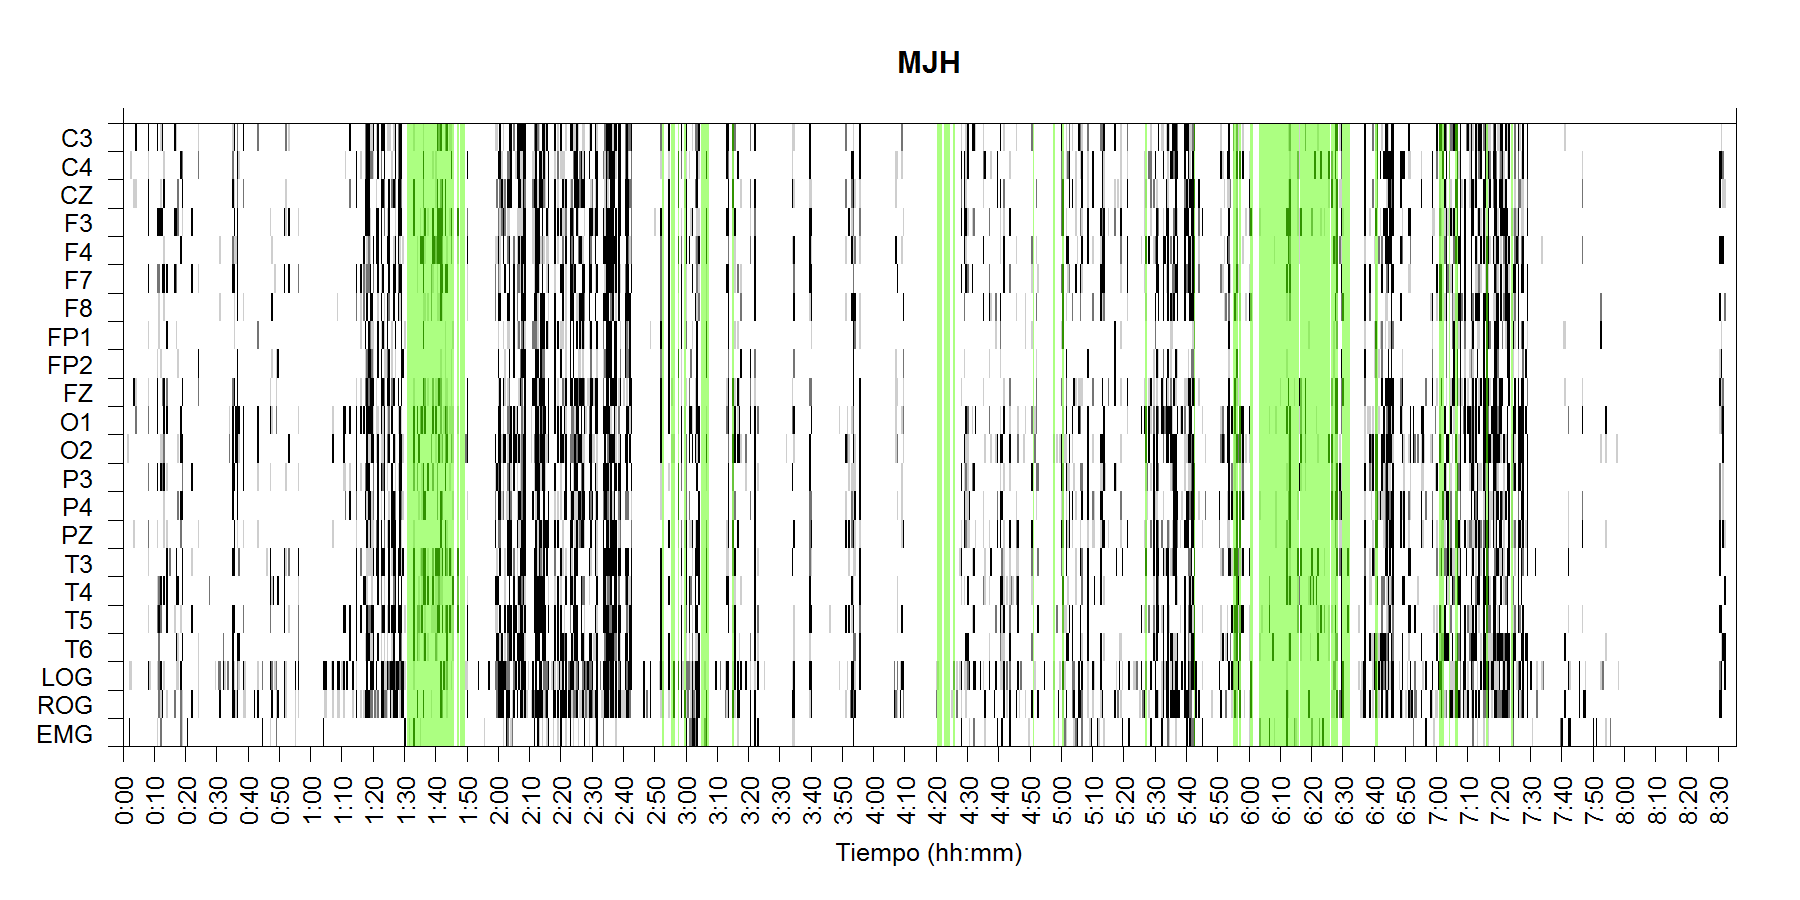
\includegraphics[width=\textwidth]{./img_ejemplos/MJNNVIGILOS_est.png}
\end{figure}
\end{frame}

%%%%%%%%%%%%%%%%%%%%%%%%%%%%%%%%%%%%%%%%%%%%%%%%%

\begin{frame}\frametitle{Efecto del tamaño de la época}
\begin{figure}
\centering
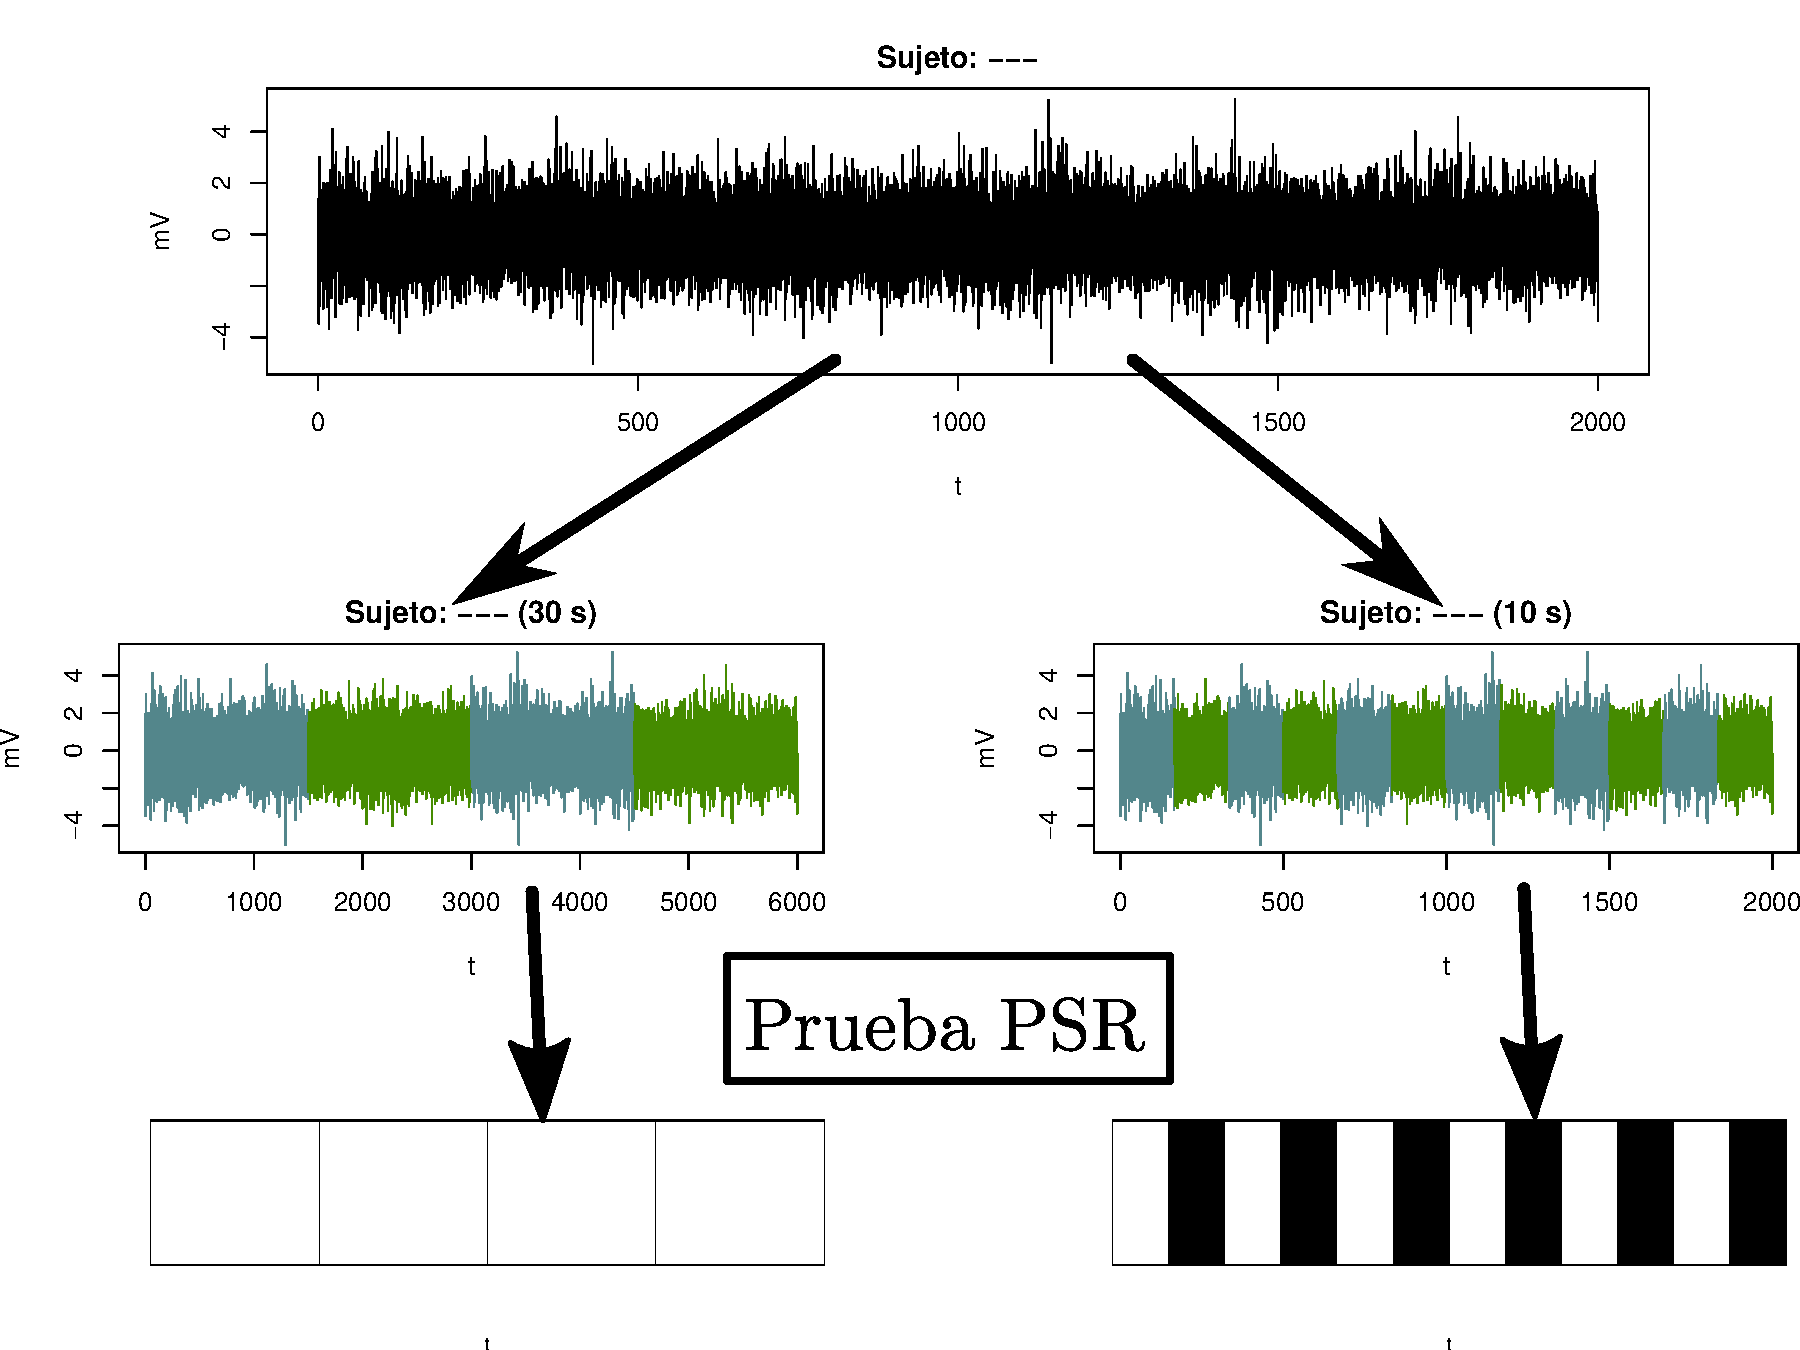
\includegraphics[width=0.9\linewidth]{./img_diagramas/epocas_diferentes.pdf}
%\caption{En el PSG}
\end{figure}
\end{frame}

%%%%%%%%%%%%%%%%%%%%%%%%%%%%%%%%%%%%%%%%%%%%%%%%%

\begin{frame}\frametitle{Efecto del tamaño de la época}
{\small Estacionariedad local\footcite{Cohen77}}
\begin{figure}
\centering
\begin{tabular}{c}
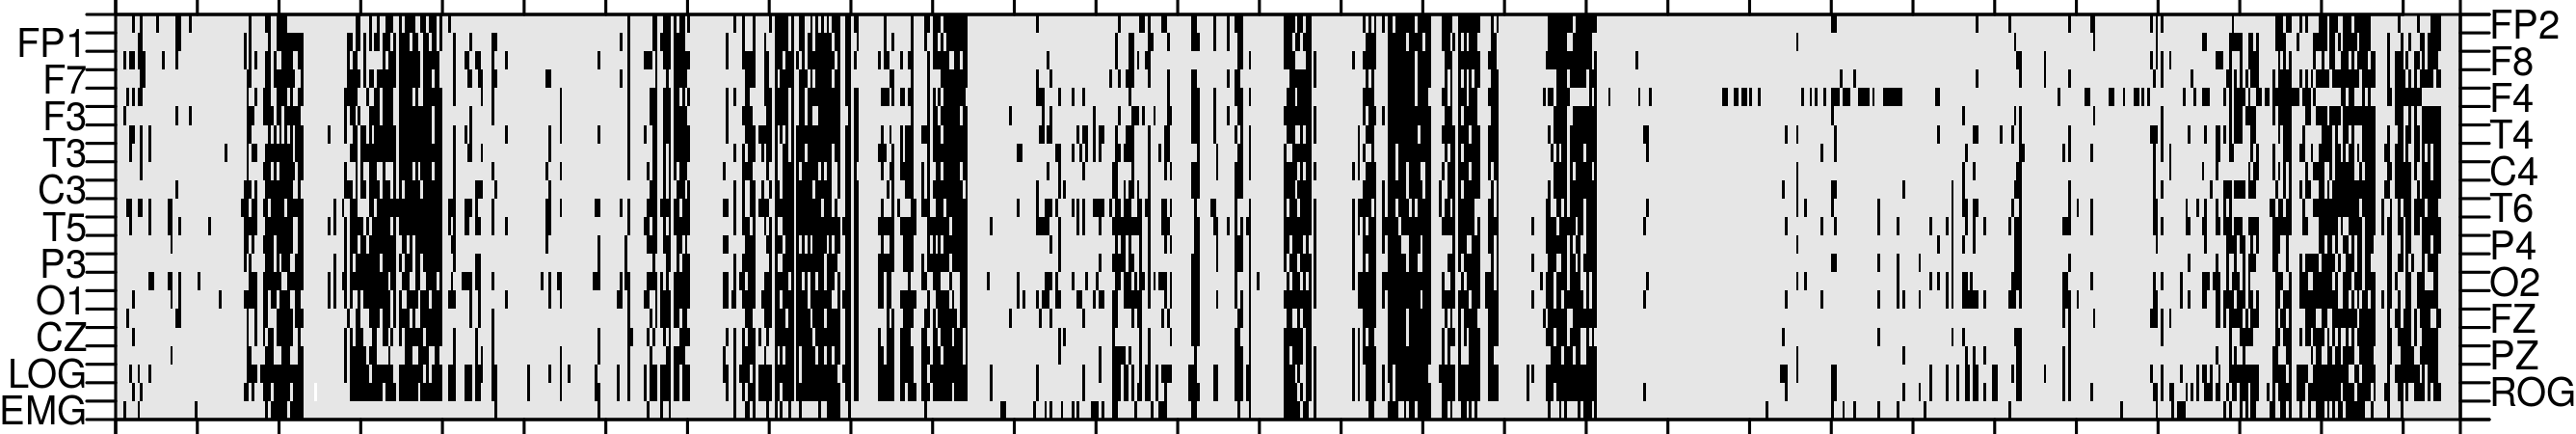
\includegraphics[width=0.4\linewidth]
{./img_ejemplos/VCNNS1_est_30.png} \\
\begin{tabular}{cc}
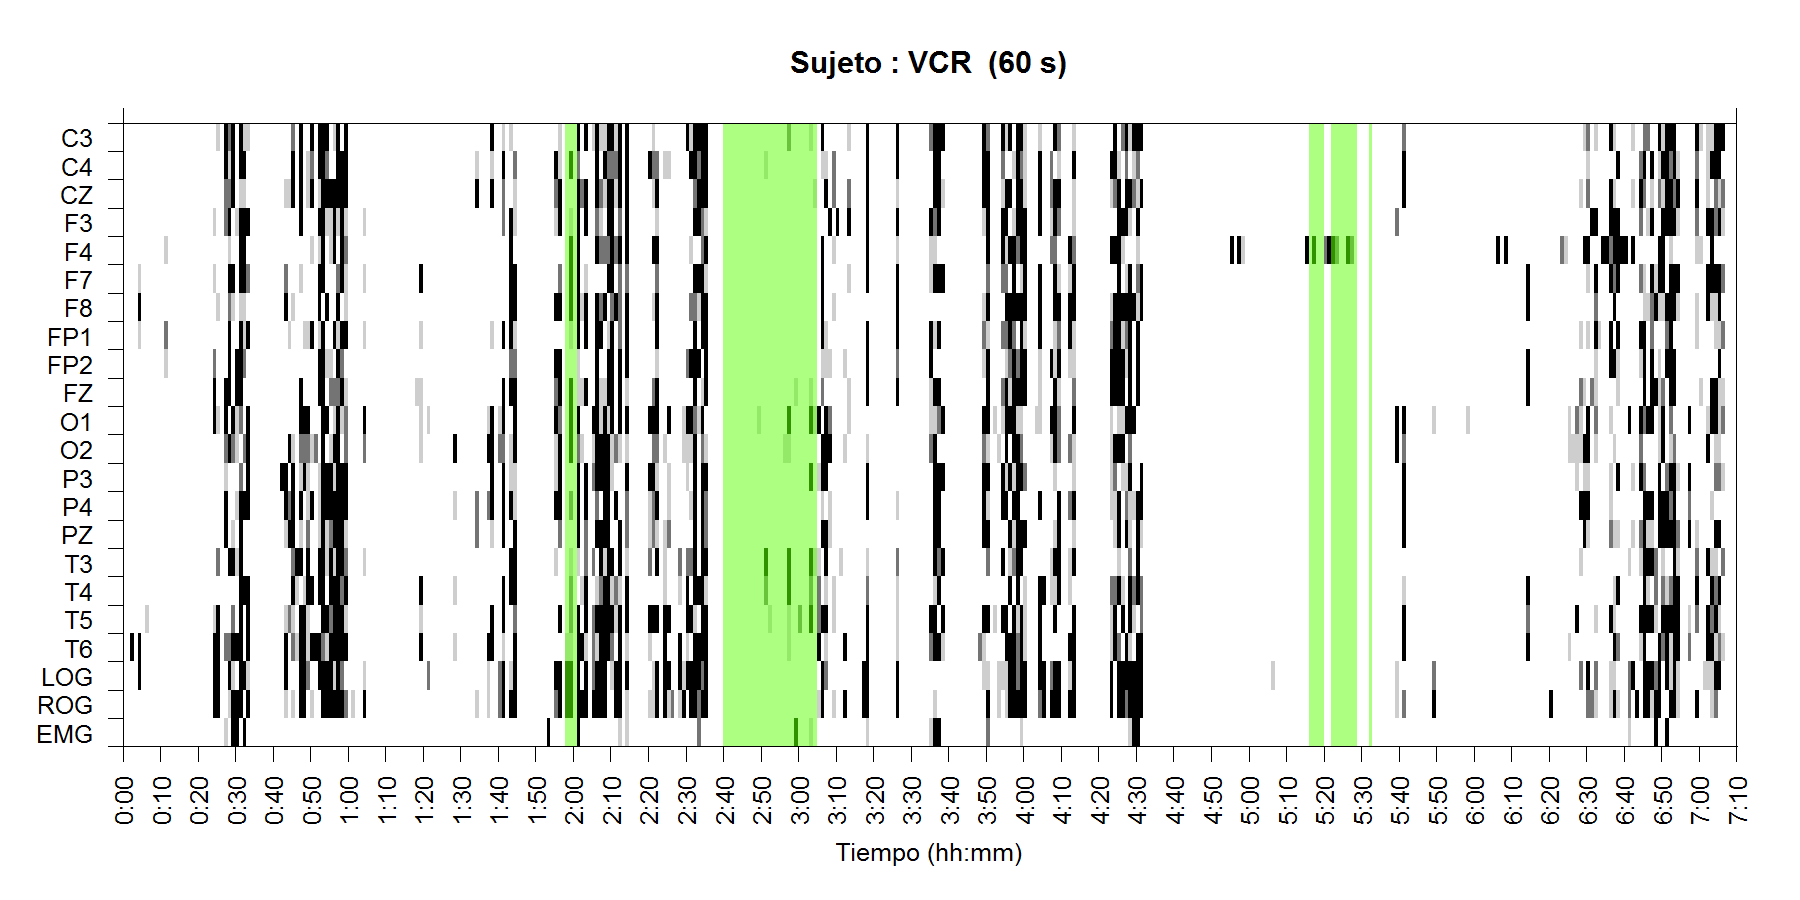
\includegraphics[width=0.4\linewidth]
{./img_ejemplos/VCNNS1_est_60.png} 
&
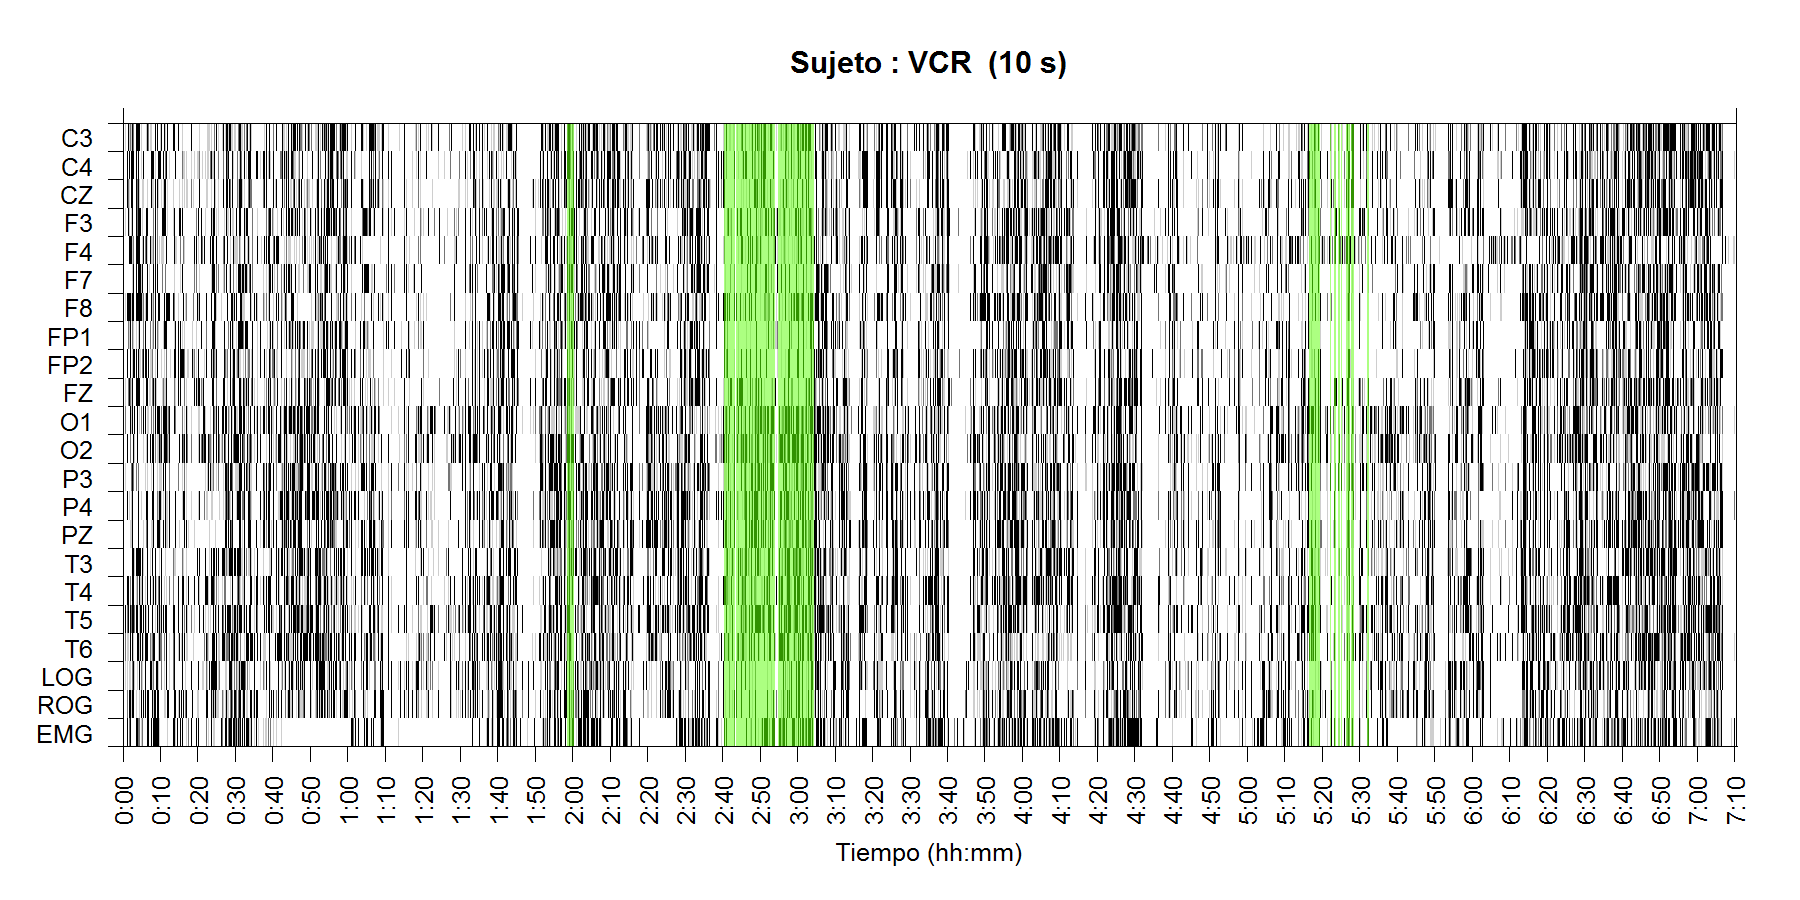
\includegraphics[width=0.4\linewidth]
{./img_ejemplos/VCNNS1_est_10.png} 
\end{tabular}
\end{tabular}
\end{figure}
\end{frame}

%%%%%%%%%%%%%%%%%%%%%%%%%%%%%%%%%%%%%%%%%%%%%%%%%

%\begin{frame}\frametitle{Gracias por su atención}
%\begin{figure}
%\centering
%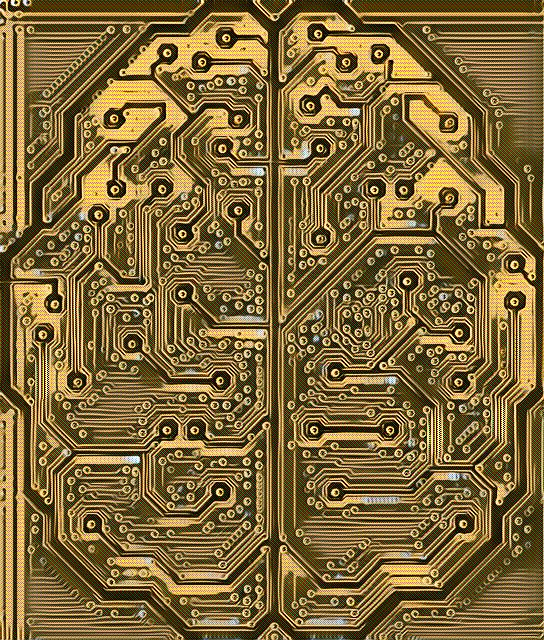
\includegraphics[width=0.4\linewidth]{./img_adornos/cerebot.jpg}\\
%\vspace*{1em}
%\textit{El cerebro es, quizá, el único órgano capaz de estudiarse a sí mismo.}
%\end{figure}
%\end{frame}

\metroset{background=dark}

\section*{Gracias por su atención}


%%%%%%%%%%%%%%%%%%%%%%%%%%%%%%%%%%%%%%%%%%%%%%%%%

\end{document}

%%%%%%%%%%%%%%%%%%%%%%%%%%%%%%%%%%%%%%%%%%%%%%%%%%%%%%%%%%%%%%%%%%%%%%%%%%%%%%%%%%%%%%%%%%%%%%%%%%%